\section{Literature Review}~\label{sec:literature}

The literature review is intended to gain an understanding of the use of classical and quantum methods in signal processing in \ac{EW}.

% Search Strategy
Involved in search strategy is the use of the Deakin Library search tool, Google Scholar, Books(accessed via library and hard-copy), and journals related to quantum computing and signal processing. 
\todo{cite: these resources}
% Search terms
% TODO: Perhaps in appendix?
% \todojc{I am not sure if it is wise to put the search keywords as part of your introduction - perhaps if your research methods chapter identifies undertaking a lit review then put these there. Also, you may need to refine these as generic terms such as "quantum computing" could help you (only because you are a novice to QC) but are not focused on the problem at hand}Search terms include:
% \begin{itemize}
%     \item Quantum Computing
%     \item Quantum signal processing
%     \item \ac{ESM}
%     \item Quantum machine learning
%     \item Quantum computing
%     \item Quantum + temporal
%     \item Software + radar
%     \item GNU Radio
%     \item Qiskit
%     \item Cognitive radar
%     \item Radar + signal processing
%     \item Temporal analysis + radar
%     \item Pulse analysis + radar
%     \item Fourier + signal processing
% \end{itemize}
% Selection criteria
Study selection criteria will be used to determine which studies are included or excluded from the review.
% Scope
\todojc{I'd leave scope to the "Scope" section}The scope of review will be used to screen studies on a per-study basis based on the whether it meets a criteria for inclusion, or exclusion.

\begin{itemize}
    \item Hardware - neither the physical implementation's of quantum nor radar will be considered.
    \item \ac{ESM}-focused. Only digitised signals to parameter estimation will be examined. Anything down-stream of identification of radar signals, (e.g., display, databasing, data fusion, etc.) and before digitisation (receive path, antennas, etc.) will be excluded
    \item \ac{SAR} and imaging radar functions
    \item Kinetic and located radar systems:
    \begin{itemize}
        \item Multi-path effects
        \item Located antennas - bi-static/multi-static, arrays
        \item Range, velocity, angle of arrival, etc.
    \end{itemize}
    \item Radar emission. Only passive, or pure \ac{ESM} scenarios will be considered
    \item Detailed radar simulation will be excluded.
    \item The range of frequency to be considered will fall within \(50MHz - 50GHz\) and be exclusive of communications signals.
    \item Adjacent problems in radar will be granted limited attention:
    \begin{itemize}
        \item Resource allocation
        \item Ambiguity analysis
        \item Tracking
    \end{itemize}
\end{itemize}

%%%%%%%%%%%%%%%%
%% Begin narrative Meta-analysis review
% Quality assesment checklist
A quality assessment checklist\cite{kitchenham_can_2010} has been adopted in order to quantitatively assess the studies based on their methodological completeness. 
% \todojc{I do not think you need to state these explicitly}
% It consists of the following questions, which will be then answered:
% \begin{enumerate}
%     \item Do the authors clearly state the aims of the research?
%     \item Do the authors describe the sample and experimental units
%     \item Do the authors describe the design of the experiment?
%     \item Do the authors describe the data collection procedures and define the measures?
%     \item Do the authors define the data analysis procedures?
%     \item Do the authors discuss potential experimenter bias?
%     \item Do the authors discuss the limitations of their study?
%     \item Do the authors state the findings clearly?
%     \item Is there evidence that the Experiment/Quasi-Experiment can be used by other researchers/practitioners?
% \end{enumerate}

% Meta-analysis
A formal meta-analysis will be conducted, and tables will be created to highlight similarities and differences among the studies.
% Classification
Each study is categorised by topic.
% Not sure if I must list them
\begin{itemize}
    \item Signal processing
    \item Time-series analysis
    \item Quantum time-series analysis
    \item Quantum encoding
    \item Quantum techniques
    \item \ac{EW}
    \item Radar techniques
    \item Radar fundamentals
\end{itemize}

The studies are also classified by methodological class \cite{wohlin_empirical_2012}.
\begin{itemize}
    \item Survey
    \item Case study
    \item Experimental
    \item Quasi-experimental
\end{itemize}

\todo{I have a table, but It seems really verbose to paste it here. It's also quite large and won't fit... see attachment 'Literature Review.xlsx'. This is effectively the meta-analysis}
\todojc{Put an improved table in the Appendix A/B/C...}
%%%%%%%%%%%%%%%%
%%% Begin narrative synthesis
%% Questions to ask:
% What is the aim of the paper?
% What are the main contributions of the paper? What new ideas are presented?
% How is the research contribution or claims justified?
% What sorts of experiments were conducted and how were the experiments set up?
% What data was obtained and how does it justify the claims made?
% Were the experiments adequate? Did they gather enough data to support the claims?
% Was data interpreted correctly? Or, Is there any explicit or hidden bias?
% Was the reasoning in the paper sound?
% What were the assumptions made in the research? Are the assumptions valid or realistic?
% How new or significant is the research idea or contribution? What are the implications to the field of the research presented?
% What are the novel aspects of the work?
% What are the shortcomings of the work? What are strengths and weakness?
% How can the work be extended or shortcomings dealt with? Does the paper encourage future work in the area?
% Are the results generalisable or applicable to another context? Are there improvements that could be made on the work?
% How is the paper relevant to your research, and how does it link to previous papers you’ve read?
%%%%%%%%%%%%%%%%

%% The problem of radar / EW
As has been illustrated, the complexity of the \ac{ESM} signal environment warrants equally complex answers to understanding it.
% Grand challenges in radar sig. proccessing / Four Problems in Radar
F. Gini \cite{gini_grand_2021} and \todojc{In addition to the listed authors, within the collection edited by Jim Barnes there also two chapters refer to quantum "things": Valeriy Labunets and then William E. Baylis, but nothing in the chapter by Wicks and Himed / or the previous Gini}\textbf{M. Wicks and B. Himed \cite{wicks_four_2004}} attempt to survey such challenges and future solutions. 
% Critique
Each survey satisfactorily outlines the challenges in the field of radar and signal processing, however both papers show a lack of rigor in experimental method, with no attempt to describe the data collection methods, selection criteria, or analysis process.
% Not academic; pragmatic.
While not useful in the academic sense, \todojc{You do not need to be apologetic for the lack of rigour, just skip all of the above and say what they say well}they do provide an illustrative overview of the emerging fields in radar engineering - waveform design, signal processing, and \ac{STAP}.
% Argument
The authors agree on a number of unanswered questions:
% Questions - not a big fan of enumerating them here.
% Q1
How to design distributed \ac{MIMO} radar to maximize detection performance and coverage area, while minimizing the revisit rate.
% Q2
How to use algorithmic hypothesis testing to merge detection and parameter estimation algorithms.
% Q3
How to better detect targets in the presence of noise and clutter by combining knowledge of signal characteristics and geometric factors.
% Q4
How to create a develop a framework for signal processing that incorporates fully adaptive transmit and receive strategies.
This last question being partially answered by contemporary cognitive radar techniques described later.

% Summary
Ultimately, both surveys underscore an urgent need for more robust, data-driven approaches to understanding the \ac{ESM} signal environment.
% Relevance
\todojc{This argument is back to front - the two cited articles do not even mention "quantum" but you write as if they did suggest this - they did not, you have not as yet motivated the need for quantum \textbf{which should be done before research question is stated} - please rephrase to make argument sound correct, e.g. something of the sort but much better: these authors recognise the complexity of the tasks ant quantum tech is good at dealing with complexity}Given the potential of quantum computing to accelerate algorithmic hypothesis testing and signal processing tasks, the authors' call for better detection and parameter estimation algorithms and signal processing frameworks presents a compelling case for exploring how quantum computing methods can be harnessed to detect and classify radar signals more effectively.

% Link. Why simple over hard problems; hedge
With the complexity of problems in the well-established field of \ac{EW} and the relative novelty of quantum signal processing, a practical approach taken is to explore this early application of quantum methods to a simpler class of radar problems.
% Non-adaptive radar types
It is important to start by examining the basic types of radar that can be used in the experiments, including Continuous Wave (CW) Radar, Frequency Modulated Continuous Wave (FMCW) Radar, Pulse Radar, Doppler Radar, Frequency Modulated Pulse (FMP) Radar, Stepped Frequency Radar, and Ultra-Wideband (UWB) Radar. \todo{use the /ac command to define each}
% Characteristics link
Each of these types of radar has unique characteristics that make them suitable for different applications, and understanding them is crucial in developing effective quantum signal processing method.

\todo{Go into each method and provide an overview. They should be cited: perhaps a survey? Perhaps ESM papers for understanding each type? There's a bit of a lack in fundamental research here...}

%% Cognitive radar
% Contrast simple radar to modern stuff
\todojc{I do not understand this here, are you talking about what was mentioned before (surely not), or do you want to refer to what you are going to say next (if so rephrase)}\textbf{Such simple and somewhat contrived examples are obviously not representative of contemporary methods}, but indeed are they necessary in undertaking such fundamental and novel research, thus in order to fully \textbf{contrast this artificiality}, we look to "cognitive radar".
%%Cognitive Radars: A Reality?
% A definition
S. Haykin describes cognitive radar as one that "continuously learns about the environment through experience gained from interactions with the environment, the transmitter adjusts its illumination of the environment in an intelligent manner, the whole radar system constitutes a dynamic closed feedback loop encompassing the transmitter, environment, and receiver" \cite{haykin_cognitive_2006}.
% A second definition
Greco et. al. \cite{greco_cognitive_nodate} concur, but stress a distinction between adaptive and cognitive radar wherein the former is constrained to receive processing only, whereas the latter includes on-the-fly intelligent transmit characteristics too.
% The need thereof
The authors' primary argument on behalf of cognitive radar is the lack of spectrum availability for traditional mono-function radars to operate.
% Comparison to other dense environment concerns
This mirrors earlier observations by M. Petterson:
\begin{quote}
    \textit{"The increased pulse density created by the deployment of pulse Doppler radar, both enemy and friendly, has created demand for systems with a high signal processing capability"}  \cite{pettersson_illustrated_1992}% p. 42
\end{quote}
% Better <-> different <==> different => quantum (:. quantum -> better)
Either high signal processing capability or different signal processing capability are needed, and if a different capability is suitable for cognitive signal processing, then so too could a different approach work for quantum signal processing.
% Critique
\todo{in progress >}
Methodologically, Greco et. al. is quasi-experimental. \todojc{Again, do not focus on what is wrong with the paper, was it important enough to include it in this review, if so just say what is its contribution to your discussion - \textbf{this applies to all the following as well!!!}}The paper lacks ...
S. Haykin's seminal work is more rigorous in research design, and when compared to the papers examined it was above average.
Haykin presents a clear and evidenced ...


\todo{    - Chapter 3 - Foundations of cognitive radar for next-generation radar systems}
\todo{:: Problem solving approaches}
\todo{:: Traditional techniques}
\todo{ Collection of techniques, used for data fusion}
\todo{    - Object Recognition and Identification Using ESM Data}
\todo{ Hardware (FPGA)}
\todo{    - Real-time radar pulse parameter extractor}
\todo{ Mathematical transform}
\todo{    - Weak radar signal detection based on wavelet transform}
\todo{ Flowchart}
\todo{    - Deinterleaving of radar signals and PRF identification algorithms}
\todo{ Mathematical transform (complex)}
\todo{    - A parameter extraction technique for FMCW radar signals using Wigner-Hough-Radon transform}
\todo{ Knowledge-based}
\todo{    - Knowledge-based Signal Processing for Radar Identification}
\todo{ ML: Basic techniques}
\todo{    - Classification of Radar Emitters Based on Pulse Repetition Interval using Machine Learning}
\todo{ Machine learning (survey)}
\todo{    - Deep-Learning for Radar: A Survey}
\todo{ DNN: }
\todo{    - A Complete Framework of Radar Pulse Detection and Modulation Classification for Cognitive EW}
\todo{ DNN - recurrent}
\todo{    - Classification, Denoising, and Deinterleaving of Pulse Streams With Recurrent Neural Networks}
\todo{:: Quantum}
\todo{    - Quantum Information Theory}
\todo{ Quantum fundementals}
\todo{    - Quantum Programming Language: A Systematic Review of Research Topic and Top Cited Languages.}
\todo{    - Qiskit: An Open-source Framework for Quantum Computing}
\todo{ Promise of quantum time-series}
\todo{    - A walk through of time series analysis on quantum computers}
\todo{ Quantum Signal processing}
\todo{    - Product Decomposition of Periodic Functions in Quantum Signal Processing}
\todo{    - Quantum eigenvalue estimation via time series analysis}
\todo{ Encoding}
\todo{    - Encoding patterns for quantum algorithms}
\todo{    - Expressibility and Entangling Capability of Parameterized Quantum Circuits for Hybrid Quantum‐Classical Algorithms}
\todo{ QNN}
\todo{    - Exponential data encoding for quantum supervised learning}
\todo{ QNN}
\todo{    - Learning temporal data with a variational quantum recurrent neural network}
\todo{:: Begin thematic synthesis}


%%%%%%%%%%%%%%%%
% Theoretical synthesis: This type of synthesis involves developing a new theoretical framework or model by synthesizing the existing literature. The authors may identify the gaps or inconsistencies in the literature and propose a new theoretical perspective.
%% Begin Critical synthesis: In this type of synthesis, the authors critically analyze the studies' methodologies, theories, and findings, and evaluate the strengths and weaknesses of the literature.




% I'm going to refactor this next bit...
\todojc{Instead of saying "Object Recognition and Identification Using ESM Data", use ref to the authors}Taghavi et al. \cite{taghavi_object_2016} present a survey of techniques in \ac{ESM} and kinematic measurement, as well as a novel approach to the fusion of the two. 
The ultimate goal of their research was recognition and identification of \todojc{You may need to say what are "targets", e.g. "identification of objects of interests in radar signals, to be later used for military targets", or whatever is appropriate}\textbf{targets}. 
The authors present a novel architecture for combining both \todojc{"approaches"?}\textbf{data-sets}, suggesting that traditional approaches or silo-ed analyses are limited. 
In the paper, they stress the importance of using orthogonal source data; that is, the inputs of the system must represent non-overlapping phenomena.

While their \todojc{You've never mentioned "problem solving"}\textbf{problem solving} methodology was novel, \todojc{What "execution"? I thought you said it was a survey? You may need to say they have also provided algorithms for different tasks? Or that the survey was limited to maritime applications}
\textbf{the execution} was somewhat limited in the respects that they restricted their simulation to the maritime domain, and with simulated data.
If their methods were to be applied practically, the limitation imposed by the maritime domain implicitly reduces the possibility for multi-path ambiguities.
The small amount of real-world data also show a systemic challenge in radar signal analysis research.
Furthermore, while their survey presented several classical approaches for the estimation of source parameters (both \ac{ESM} and kinematic), the methods were only analytical.
There was no mention of machine learning-based recognition and identification frameworks. The analytical methods presented were generally applicable and relevant for a baseline of ESM techniques.
For example: Bayesian framework, belief functions, fuzzy set theory.
The data-fusion framework presented in the paper does provide an applicable architecture for multi-domain analysis which may prove useful in future research.
% Maybe I should make this more relevant to the problem at hand? Like drawing parralels to the challenges and approaches suggested for our research. % On second thought, each such analytical method should be explained 

Geng et al. \cite{mason_deep_2017} provide a broad outlook on the current state of affairs in the use of deep learning in radar signal processing. The authors analysed a large body of research over several areas of radar signal processing and for a multitude of deep learning techniques. The paper identifies numerous applicable approaches with varying degrees of effectiveness. Deep learning techniques discussed were:
\begin{itemize}
 \item \todojc{Are they all relevant to radar signal processing? If so briefly state how}CNN: Convolutional neural network
 \item DBN: Deep belief network
 \item DRL: Deep reinforcement learning
 \item DRES: Deep residual neural network
 \item FNN: Feed-forward neural network
 \item GAN: Generative adversarial network
 \item RNN: Recurrent neural network, including long-short term memory
 \item SAE: Stacked auto-encoder
\end{itemize}

The methods analysed in the paper, while comprehensive overall, still failed to attack the problem of parameter estimation. 

Several limitations were also identified, some being systemic to the field, others specific to deep learning techniques. Some challenges identified were \todojc{What does it mean?}their \textbf{subjectivity to Electronic Attack (EA)}, where, depending on the level of intelligence about the Deep Neural Networks (DNN) techniques employed, various exploitations may be executed. Of course, EA is not specific to DNN's, however, it's noted that because they exist as an heuristic model, they necessarily have gaps in their model of the problem space. Therefore, it's noted that DNN's may be more suseptable to EA because of its inherent non-analytical method. Similar to Taghavi et. al. the lack of training data is a serious challenge in the testing and validation of any radar analysis model. This proves a large problem in any future effor for open-source development of DNN's for radar analysis, as noted by the authors that DNN's require large amounts of training data. The paper concludes with an evaluation of particularly effective methods, some reaching > 97\% accuracy, however as described - with small training sample sizes.

The primary interest of \todojc{which option? DNN?}\textbf{this option} is in passive radar, i.e., radars which generally do not transmit energy and listen to a return. An example is a Radar Warning Receiver (RWR) which is a passive electronic warfare support system \cite{avionics_department_electronic_2013}

One functional mode of RWR's is the search mode: where the system’s objective is to interrogate the electromagnetic environment to detect and identify emitters. The only information that radars are given is the signals which it receives, and its location in space and time (as well as some prior understanding of the operational environment). Due to the nature of the operating context, modern radars may receive many incident signals in a short period of time. Within such received signals, there may exists a number of constituent parts: communications signals, radar signals, interference (whether intentional or not), and noise (being environmental, or system). For signals originating from radars, they vary in several dimensions: see radar domains. Noise is generally constant, but limits the receiver’s ability to detect a given signal’s presence. Interference is any signal which interferes with the receiver’s ability to perform its function – either fully or partially. The functional operation of the receiver is: signal input (coming from antenna), RF front-end, digitisation, and processing. In each stage, the signal may change characteristics and formats based on a variety of filtering and processing operations. \cite{stimson_introduction_1998}\todo{This last one needs to be refined and specified to more constraints / trade-offs of radar I think.}

"Encoding patterns for quantum algorithms" - Weigold et.al. \cite{weigold_encoding_2021} details several applicable approaches to encoding data for quantum algorithms. The problem presented in the paper is that quantum computing may have (in some cases) exponential speed-up when compared to classical methods, however data loading is often inefficient. Starting with a description of the quantum format itself, (qubits), the paper implicitly shows how quantum methods differ from classical formats through an explanation of the former. The substance of the article then goes on to focuses on a comparison of practical means of transforming data, specifically:
\begin{itemize}
 \item Basis encoding
 \item Angle encoding
 \item QuAM encoding 
 \item QRAM encoding
 \item Amplitude encoding
\end{itemize}

The paper comprehensively details each approach, their applications, methods, and variants.
Interestingly, the authors also present four methods on quantum state preparation, such that once data are loaded from their classical sources, that they may be prepared for quantum operations.
The approaches covered were:

\begin{itemize}
 \item Schmidt decomposition
 \item Matrix encoding
 \item Quantum Phase Estimation
 \item Post-selective measurement
\end{itemize}

\todojc{I agree with your hidden notes on the need for more synthetic lit review}
\todojc{And, it would be great to have a conceptual model - which could be visual / tabular / descriptive - at the end to show how all of the more important domain concepts are inter-related, how the quantum solution / your research question fits into it, which aspects are within the scope and what is outside the scope. Also note that any figure needs a description in text, and so would the model!}
\todojc{Note that the body of knowledge summarised here would be drawn from your Introduction / Background / and Lit Review}
Finally, an example solution to the well known quantum algorithm for linear systems of equations - the HHL algorithm - using several of the mentioned approaches were compared.

Overall, the paper makes a comprehensive survey of encoding approaches with strong analytical grounding. The approaches mentioned, while soundly applicable to many forms of atomic classical data, somewhat neglect the complexity of real-world data. A specific example would be high-dimensional timeseries (as is used for radar signal processing), which neither classical computing nor quantum computing have yet to represent faithfully. Such a limitation may be simply a result of the technologies used, rather than the methods presented in this article. The paper effectively describes and identifies the benefits and limitations of each method in terms of efficiency and entropy conversion trade-offs.

\todojc{Text in diagram not readable}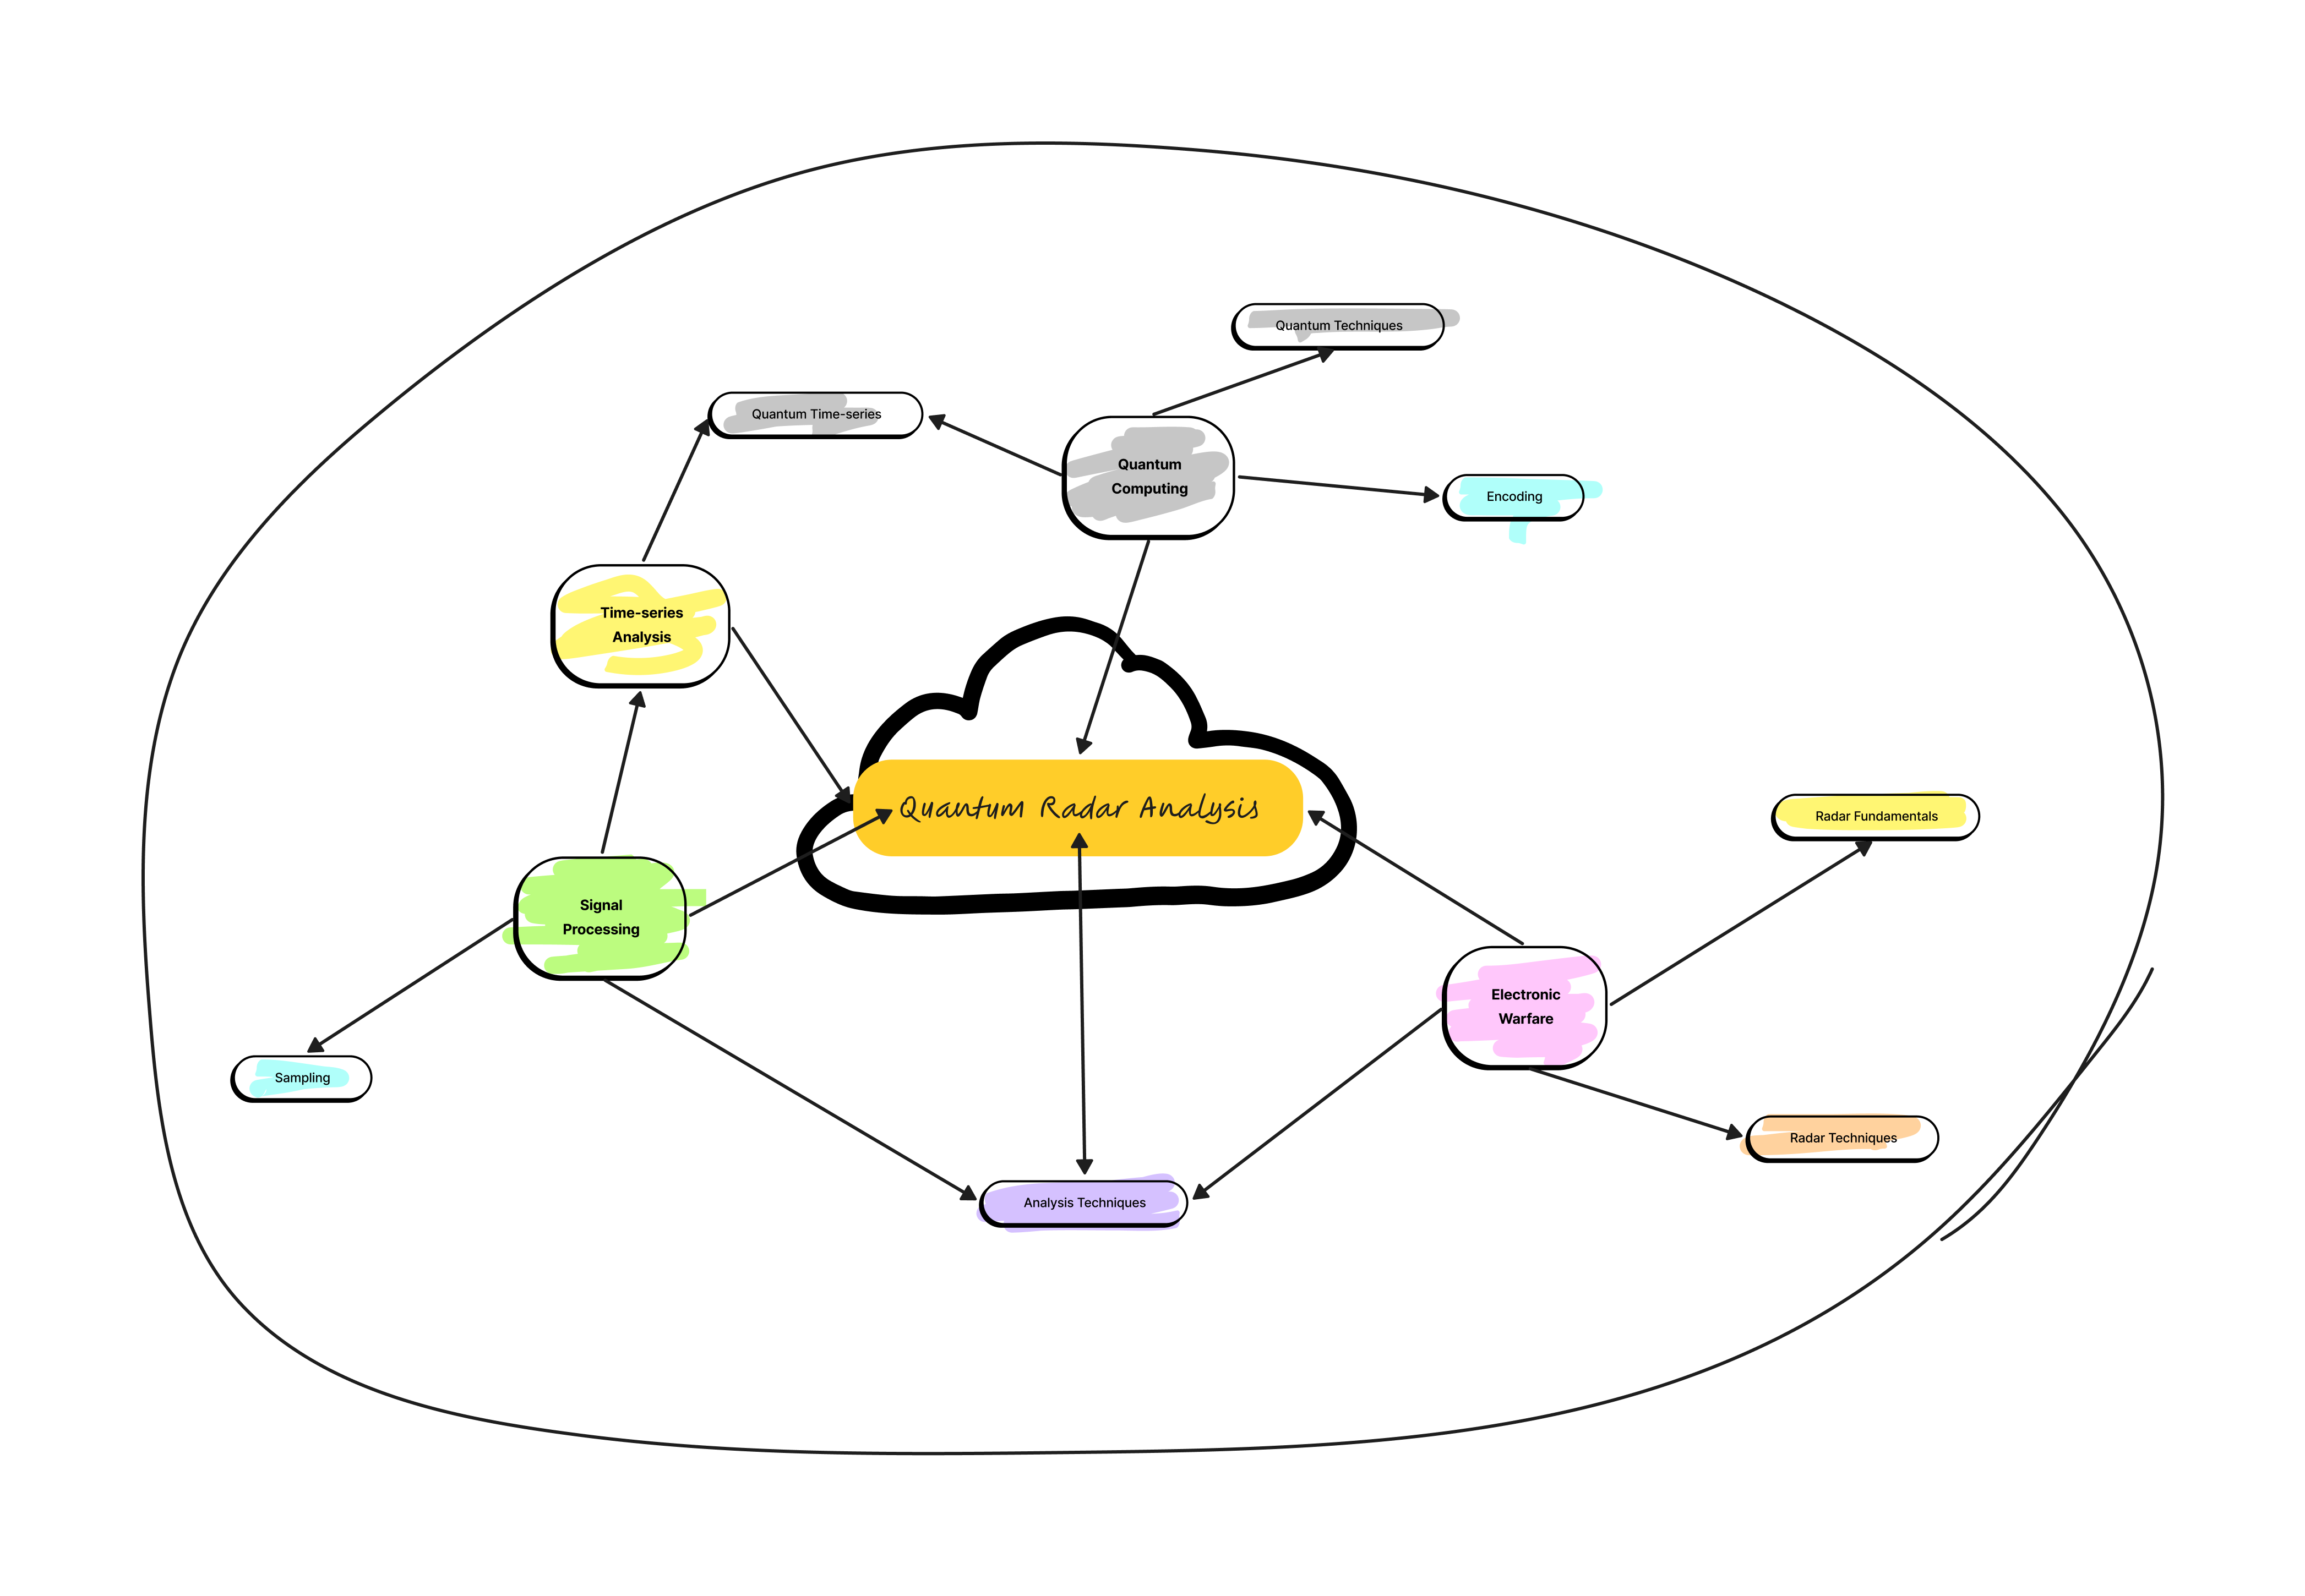
\includegraphics[width=1\textwidth]{Figures/Literature review - mind map.png}
\todo{caption and description}
\todojc{\textbf{At the moment the review is bleeding with great effort and severe hardship, and reads like this. You introduce each paper as a separate entity and first describe it as a research project, then whether it is good or bad, what is bad and what is good, and sometimes you even say what is relevant to your line of argument. As is there is no story to tell! It would be better to simply talk about radar signal processing and as part of your story bring in ideas from those papers. Quantum tech for radar signal processing should emerge naturally as part of the argument, which should show how people approach radar signal processing, what was really hard, and that quantum tech is good at what was hard, so it would be worth trying it out}}

\subsection{Gap-analysis}

% Quantum
A large body of research has been conducted into quantum computing, with many papers focusing on quantum problem solving methods and encoding.
Furthermore, the realm between that, and of signal processing have been explored to a lesser degree.
However, the niche of encoding time-series sampled data (as what will be required in this research) has only been explored in more limited respect.
From the perspective of method, many studies in quantum computing were found to lacked methodological precision.

% Radar
The field of radar too has been extensively explored over many previous decades.
Many studies have explored the fine details of radar techniques, few studies clearly defined simpler approaches in radar.
While there is a wealth of literature on radar processing, the gap exists not in the field as it stands, however in the lack of contra-normative methods, like quantum computing.

Given these insights, it was found that little available research exists on the fusion of radar/\ac{EW}, signal processing, and quantum computing - despite large bodies of research existing in each respective field alone.
Therefore this combination is the line of enquiry this research will address.
% Additionally, this study aims to address the general deficiency in methodological rigor, of which both principal areas of interest were found to lack.

% NOTES FROM MEETING 1
% 1. Academic references - explain / summarise them\\
% 2. Develop a meta-model of their fundamental argument, challenges, deficiencies, and strengths\\
% 3. Compare their differences, similarities, and whether or not they agree. (If they all agree, more sources should be found); how they interrelate.\\
% 4. Next, the exposition of the problem space (radar signal analysis) should be written, being lean enough so as to only explain the content of the referenced academic sources. I.e., the challenges faced should be fully developed.\\
% 5. Following which, a more precise formulation of problems should be undertaken.

% Here are some ones I would like to properly analyse in more depth (not yet added to Zetaro)
% - https://ietresearch.onlinelibrary.wiley.com/doi/pdf/10.1049/iet-rsn.2017.0516
% - https://ietresearch.onlinelibrary.wiley.com/doi/pdf/10.1049/iet-rsn.2017.0563
% - Improvements on deinterleaving of radar pulses in dynamically varying signal environments: Kenan Gençol, Ali Kara, Nuray At (2017)
% - Estimating the Instantaneous Frequency of Linear and Nonlinear Frequency Modulated Radar Signals — A Comparative Study Hubert Milczarek, Czesław Le´snik, Igor Djurovi, and Adam Kawalec
